% \documentclass{article}
% %\usepackage[english]{babel}%
% \usepackage{graphicx}
% \usepackage{tabulary}
% \usepackage{tabularx}
% \usepackage[normalem]{ulem}
% \usepackage{cancel}
% \usepackage{tikz} 
% \usepackage{pdflscape}
% \usepackage{colortbl}
% \usepackage{lastpage}
% \usepackage{multirow}
% \usepackage{enumerate}
% \usepackage[shortlabels]{enumitem}
% \usepackage{color,soul}
% \usepackage{pdflscape}
% \usepackage{hyperref}
% %\usepackage[table]{xcolor}
% \usepackage{rotating}
% \usepackage{amsmath}
% \usepackage{fixltx2e}
% \usepackage{framed}
% \usepackage{mdframed}
% \usepackage[T1]{fontenc}
% \usepackage[utf8]{inputenc}
% \usepackage{textcomp}
% \usepackage{siunitx}
% \usepackage{ifthen}
% \usepackage{fancyhdr}
% \usepackage{gensymb}
% \usepackage{newunicodechar}
% \usepackage[document]{ragged2e}
% \usepackage[margin=1in,top=1.1in,headheight=57pt,headsep=0.1in]
% {geometry}
% \usepackage{ifthen}
% \usepackage{fancyhdr}
% \everymath{\displaystyle}
% \usepackage[document]{ragged2e}
% \usepackage{fancyhdr}
% \everymath{\displaystyle}
% \usepackage{empheq}

% \usepackage[most]{tcolorbox}

% \usepackage{booktabs} % Required for nicer horizontal rules in tables


% \usepackage{enumitem}

% %\usepackage[table,xcdraw]{xcolor}
% \usetikzlibrary{arrows}
% \linespread{2}%controls the spacing between lines. Bigger fractions means crowded lines%
% %\pagestyle{fancy}
% %\usepackage[margin=1 in, top=1in, includefoot]{geometry}
% %\everymath{\displaystyle}
% \linespread{1.3}%controls the spacing between lines. Bigger fractions means crowded lines%
% %\pagestyle{fancy}
% \pagestyle{fancy}
% \setlength{\headheight}{56.2pt}

% \definecolor{myblue}{rgb}{.8, .8, 1}
% \newcommand*\mybluebox[1]{%
% \colorbox{myblue}{\hspace{1em}#1\hspace{1em}}}

% \chead{\ifthenelse{\value{page}=1}{
\includegraphics[scale=0.3]{SCC}\\ \textbf \textbf Wastewater Constituents Analysis \& Laboratory Methods}}
% \rhead{\ifthenelse{\value{page}=1}{}{}}
% \lhead{\ifthenelse{\value{page}=1}{}{Wastewater Constituents Analysis \& Laboratory Methods}}
% \rfoot{\ifthenelse{\value{page}=1}{Module 1: WATR 048 - Spring 2019}{Module 1: WATR 048 - Spring 2019}}

% \lfoot{Shabbir Basrai}
% \cfoot{Page \thepage\ of \pageref{LastPage}}
% \renewcommand{\headrulewidth}{2pt}
% \renewcommand{\footrulewidth}{1pt}
% \begin{document}
% %\begin{empheq}[box=\mybluebox]{align}
% %a&=b\\
% %E&=mc^2 + \int_a^a x\, dx
% %\end{empheq}

% \newlist{steps}{enumerate}{1} % Defines "Steps" for enumerate as Step 1, Step 2 etc.
% \setlist[steps, 1]{label = Step \arabic*:} % Defines "Steps" for enumerate as Step 1, Step 2 etc.

% \setlist{nolistsep} % Reduce spacing between bullet points and numbered lists


%_______________________________________________________________________________________________________________________________________%
\chapterimage{IntroductionSecondaryTreatmentImage.jpg} % Chapter heading image

\chapter{Introduction to Secondary Treatment}
\begin{itemize}
\item While preliminary and primary treatment processes are designed primarily to remove solids from wastewater, secondary treatment is for the removal of organics.
\item Secondary treatment involves:
\begin{itemize}
\item biological conversion of the dissolved and suspended organics in wastewater into biomass, and
\item physical settling (separation) process where the solids including the biomass formed during secondary treatment is separated and removed from the treated wastewater.
\end{itemize}

\item With the removal of gross solids in the preliminary treatment followed by removable of settleable solids in the primary clarifiers and the removal of dissolved and suspended organics in the secondary treatment processes, the wastewater is considered treated.
\item Secondary treated wastewater is typically disposed or treated further for reuse or disposal (depending upon the end use/application and the NPDES permit stipulations).
\item The solids (biomass) removed from the secondary treatment is typically mixed with the solids from primary treatment and stabilized using a solids treatment process like sludge digestion prior to its disposal.
\end{itemize}
\vspace{1cm}

\textbf{Secondary treatment process incorporates one of the following three approaches:}


\section{Fixed film system}\index{Fixed Film System}	

\begin{itemize}
\item Here the microorganisms responsible for the treatment, grow on substrates such
as rocks, sand or plastic.
\item When the wastewater is spread over the substrate, the microorganisms up-take the organics present in the wastewater
\item Example of this secondary treatment process include trickling filters and rotating biological contactors\\
\end{itemize}

\section{Suspended Growth System}\index{Suspended Growth System}
\begin{itemize}
\item In this type of secondary treatment, the microbes are suspended in the
wastewater flow being treated. 
\item Air or oxygen is supplied to maintain an aerobic environment and to keep the microorganisms in suspension. 
\item Example of this secondary treatment approach include the activated sludge treatment process 
\end{itemize}

\section{Pond System}\index{Pond System}
Similar to the suspended growth, stabilization ponds are large man made bodies of water which treat wastewater using mainly natural processes including sunlight, algae and microorganisms.




\chapterimage{TFChapterImage1.jpg} % Chapter heading image

\chapter{Trickling Filters}




\section{Theoretical Background}\index{Theoretical Background}
		
Trickling filter is a fixed film secondary treatment process wherein the organic content of the wastewater is removed using biological growth attached to an inert media such as lava rock or plastic\\			
\begin{itemize}
\item In a trickling filter, the wastewater is sprayed evenly on the surface of the media with a rotary type distributor with orifices
\item The wastewater percolates through the media bed, where it comes in contact with biological slime growth – zoogleal film (zooglea)
\item The aerobic biomass - bacteria, protozoa and other microoorganisms in the zooglea capture and consume the suspended and dissolved organics from the wastewater.
\item The microorganisms metabolize the organics and in the process produce more microbial mass resulting in increasing the thickness of the zoogleal layer.
\item The thickness of the zoogleal layer can only increase to a point until the wastewater flow – hydraulic load, shears the slime layer – “sloughs off” and is carried out as part of the effluent flow as sloughing.
\item The treated wastewater cascades from the bottom of the media into the underdrain system – lower portion of the TF comprised of columns which support the media base.  The underdrain has a sloping floor to direct the cascading water into a center channel .
\item The clarifier allows for the separation (settling) of the  of the solids (sloughed off material).  The settled solids is removed - typically pumped to a digester and the clarified effluent flows out of the clarifier.
\item The source of oxygen to support the aerobic growth is from the oxygen dissolved in the wastewater as it is sprayed over the media and from the air currents due to the downward flow of the wastewater and the temperature difference between ambient and the interior of the trickling filter.  Forced ventilation system may be designed as part of the trickling filter

\item Word trickling “filter” is a misnomer - no filtration is involved
\item Advantage includes process simplicity and lower costs
\item Disadvantage include BOD removal efficiency of only about 80-85%
\item The media may be rock, slag, coal, bricks, redwood blocks, molded plastic, or any other sound durable material.
\item The media depth ranges from about three to eight feet for rock media trickling filters and 15 to 30 feet for synthetic media.
\item The media needs to be uniformly sized and have adequate empty spaces (voids) to ensure maintaining aerobic condition necessary for the survival of biomass.  

\item Pre-fabricated (synthetic) media - similar to the one shown below, has an advantage over the "dumped" type media such as lava rock of providing a greater surface area per volume upon which the zoologeal film may grow while providing ample void space for the free circulation of air.

\item Sometimes, due to inadequate hydraulic loading, portions of the zoogleal layer may become too thick and oxygen cannot penetrate its full depth, causing odor issues.

\end{itemize}


\section{Trickling Filter Recirculation}\index{Trickling Filter Recirculation}

Recirculation - where a portion of the treated wastewater is returned back as the feed to the TF.  The parameter recirculation ratio is calculated to quantify the recirculation flow.  Recirculation ratio is a ratio of the recirculated flow - Q$_R$ to the influent flow Q$_I$. Recirculation ratios typically vary from 0.5 to 4.
\begin{center}
\includegraphics[scale=0.5]{TFrecirculation}
\end{center}
Recirculation is beneficial for the following reasons:
\begin{itemize}
\item It improves the removal efficiency by increasing the contact time of the zoogleal layer with the wastewater
\item During low flows it prevents the trickling filter from drying out
\item It dilutes any toxic loadings
\item It promotes oxygen transfer and reduces ponding
\item The increased hydraulic loading promotes uniform sloughing, prevents ponding, improves ventilation through the filter and reduces potential for snail and filter fly breeding
\end{itemize}
\section{Operation of Multiple Trickling Filters}\index{Operation of Multiple Trickling Filters}

Multiple trickling filters can be operated in series or in parallel:\\
\begin{itemize}
\item Series operation in which the flow from one flows into the next.
\begin{center}
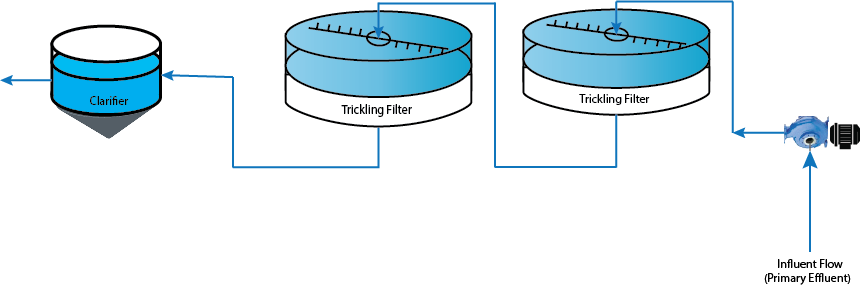
\includegraphics[scale=0.5]{TFSeries1}
\end{center}  
\begin{itemize}
\item For high strength loading and for nitrification
\end{itemize}
\item Parallel operation in which the trickling filters that are operated side by side.
\begin{center}
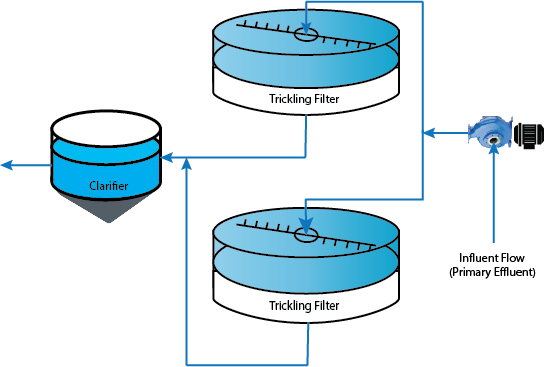
\includegraphics[scale=0.6]{TFParallel1}
\end{center}
\begin{itemize}
\item For winter operation - prevents freezing in the TF
\end{itemize}
\end{itemize}

\section{Parameters for monitoring and operating trickling filters}\index{Parameters for monitoring and operating trickling filters}



\begin{enumerate}
\item Hydraulic loading is expressed as gpd/$ft^2$
\item BOD Removal (\%)
\item Organic loading lbs BOD/day/ 1000 cu ft
\item Recirculation ratio
\end{enumerate}


\section{Classifying Trickling Filters}\index{Classifying Trickling Filters}			
Trickling filters are classified according to the hydraulic and organic loading applied to the  filter\\

\subsection{Low-rate filter}\index{Low-rate filter}

\begin{itemize}
\item The standard rate or low rate trickling filters (LRTF) are relatively simple treatment units that normally produce a consistent effluent quality even with varying influent strength
\item They are generally not provided with recirculation of effluent
\item Depending upon the dosing system, wastewater is applied intermittently with rest periods which generally do not exceed five minutes at the designed rate of waste flow. 
\item While there is some unloading or sloughing of solids at all times, the major unloadings usually occur several times a year for comparatively short Periods of time.
\end{itemize}

     Hydraulic loading is 25 - 100 gal/day/sq. ft\\
     BOD Removal (\%) 	50 – 80\%\\
     Organic loading is 5 - 25 lbs BOD/day/1000 cu ft\\

\subsection{High-rate filter}\index{High-rate filter}

\begin{itemize}
\item The most important element of a high-rate trickling filter is the provision where a part of the settled treated effluent is pumped to the PST or to the filter.  This is termed as \textbf{Recirculation}
\item High-rate filters are usually characterized by higher hydraulic and organic loadings than low-rate filters
\item The higher BOD loading is accomplished by applying a larger volume of waste per unit surface area of the filter.  \item As a result of the higher flow velocities a more continuous and uniform sloughing of excess zoogleal growth occurs
\end{itemize}

     Hydraulic loading is 100 - 1000 gal/day/sq. ft\\
     BOD Removal (\%) 	65 - 85\%\\
     Organic loading is 25 - 100 lbs BOD/day/ 1000 cu ft\\
			
\subsection{Roughing filter}\index{Roughing filter}

\begin{itemize}
\item Roughing filters are high rate type filters designed with plastic packing
\item In most cases roughing filters are used to treat wastewater prior to secondary treatment
\item One of the advantages of roughing filter is low energy requirement for BOD removal of high strength wastewaters as compared to activated sludge process because the energy required is only for pumping the influent wastewater and recirculation flows
\end{itemize}



\section{Trickling Filter Operational Issues}\index{Trickling Filter Operational Issues}

\subsection{Ponding}\index{Ponding}


If the voids in the media get plugged, flow can collect on the surface in ponds.
Correction:
spraying the surface with high pressure water stream
stopping a rotary distributor over the ponded area
hand-stir the media or open the voids
dose the filter with chlorine for several hours

\subsection{Odors}\index{Odors}


\begin{itemize}
\item Corrective measures should be taken immediately if foul odors develop
\item presence of foul odors indicates anaerobic conditions are predominant
\item Check the under drain system for obstructions or heavy biological growths
\item increase the recirculation rate to provide more oxygen to the filter bed and increase sloughing 
\item keep slime growths off of sidewalks and inside walls of the filter to reduce the odor
\end{itemize}

\subsection{Trickling Filter Flies - Psychoda}\index{Trickling Filter Flies - Psychoda}

\begin{itemize}
\item tiny, gnat-size filter fly, or Psychoda - primary nuisance insect
\item Correction methods include
\begin{itemize}
\item Increase recirculation rate
\item keep orifice openings clear
\item apply insecticides to filter walls
\item dose filter with chlorine
\item keep weeds and tall grass cut around filter
\end{itemize}
\end{itemize}


\subsection{Cold weather problems}\index{Cold weather problems}

\begin{itemize}
\item ice can form on the media of the filter
\item Correction methods include:
\begin{itemize}
\item decrease recirculation to the filter (influent is usually warmer than recycled flows)
\item construct wind screens
\item operate two-stage filters in parallel rather than in series
\end{itemize}
\end{itemize}


\section{Math Problems}\index{Math Problems}

Trickling filter problems involve calculation of the following:

\subsection{Hydraulic or surface loading}\index{Hydraulic or surface loading}

\begin{itemize}
\item Hydraulic or surface loading is expressed as gpd/$ft^2$
\item \hl{The gpd is the total flow (Q$_T$)to the filter - primary influent flow + recirculated flow(Q$_T$= Q$_I$ + Q$_R$)}\\
\end{itemize}
			\hl{Example Problem:}\\
The total influent flow (including recirculation) to a trickling filter is 1.89 MGD. If the trickling filter is 80 ft in diameter, what is the hydraulic loading in gpd/sq ft on the trickling filter?\\
\vspace{0.2cm}
Solution:\\
\vspace{0.2cm}
$Hydraulic \enspace loading \enspace \dfrac{gpd}{ft^2}=\dfrac{(1.89*10^6)gpd}{(0.785*80^2)ft^2} =\boxed{376\dfrac{gpd}{ft^2}}$
			
			
\subsection{BOD and TSS Removal}\index{BOD and TSS Removal}
BOD and  removal is based upon the TF influent and effluent concentrations.\\
\vspace{0.2cm}
$\% Removal=\dfrac{In_{conc}-Out_{conc}}{In_{conc}}*100$\\
			\hl{Example Problem:}\\
The suspended solids concentration entering a trickling filter is 236 mg/l. If the suspended solids concentration of the trickling filter effluent is 33 mg/l, what is the suspended solids removal efficiency of the trickling filter?\\
\vspace{0.2cm}
Solution:\\
\vspace{0.2cm}
$\% Removal=\dfrac{236 mg/l-33 mg/l}{236 mg/l}*100=\boxed{86\%}$

\subsection{Organic Loading}\index{Organic Loading}

			\begin{itemize}
\item Organic loading to a trickling filter is typically expressed as lbs BOD/(day-1000 cu ft).  \item The lbs/day BOD value is the BOD loading from the primary effluent.
\item The 1000 ct. ft is the volume of the media.  
\item The media volume is calculated by multiplying the TF surface area by the media height.  
\item As the dimensions are typically given in ft., calculate the volume in $ft^3$ and then divide the calculated volume by 1000 to give the volume in units of 1000$ft^3$\\
\end{itemize}
\hl{Example Problem:}\\
A trickling filter, 70 ft in diameter with a media depth of 6 ft, receives a flow of 0.78 MGD. If the BOD concentration of the primary effluent is 167 mg/L, what is the organic loading on the trickling filter in lbs BOD/day/1000 cu ft?\\
Solution:  $Organic \enspace loading:\dfrac{lbs \enspace BOD}{day-1000ft^3}=\dfrac{lbs \enspace BOD \enspace feed \enspace to \enspace TF \enspace per \enspace day}{volume \enspace in \enspace 1000ft^3}$\\
$=\dfrac{\dfrac{(0.78*167*8.34)lbs \enspace BOD}{day}}{(0.785*70^2*6)ft^3*\dfrac{1000ft^3}{1000ft^3}}=\boxed{\dfrac{47 lbs \enspace BOD}{day-1000 ft^3}}$

\subsection{Recirculation Ratio}\index{Recirculation Ratio}


$Recirculation \enspace Ratio (R_R)=\dfrac{Recirculated \enspace Flow (Q_R)}{Influent  \enspace  Flow (Q_I)}$\\
\vspace{0.5cm}
$Recirculation \enspace Ratio (R_R)=\dfrac{Total \enspace Flow (Q_T) - Influent \enspace Flow (Q_I)}{Influent  \enspace  Flow (Q_I)}$\\
\vspace{0.5cm}
$Total \enspace Flow (Q_T) = Influent \enspace Flow (Q_I)*(Recirculation \enspace Ratio(R_R) +1)$
Make sure $Q_R$, $Q_T$ and $Q_I$ units are the same in a given problem

\hl{Example Problems:}\\
\begin{enumerate}
\item The influent to the trickling filter is 1.61 MGD. If the recirculated flow is 2.27 MGD, what is the recirculation ratio?\\
\vspace{0.2cm}
Solution:  $R_R=\dfrac{Q_R}{Q_I}=\dfrac{2.27}{1.61}=\boxed{1.4}$\\
\vspace{0.2cm}
\item A trickling filter has a total flow of 32 MGD.  If the recirculation ratio is 0.8, what is the primary effluent flow to the TF?\\
\vspace{0.2cm}
Solution:\\
\vspace{0.2cm}
$Total \enspace Flow (Q_T) = Influent \enspace Flow (Q_I)*(Recirculation \enspace Ratio(R_R) +1)$\\
$\implies 32 MGD=Q_I*(0.8+1)\implies Q_I=\dfrac{32}{1.8}=\boxed{17.8 MGD}$
\end{enumerate}
\newpage
\chapterimage{QuizIcon.jpg}
\chapter{Week 4 Module Assessment Quiz}

1. The main purpose of the trickling filter media is to provide nutrients to the zoogleal mass growing on it\\

a. True \\
b. False \\
\vspace{0.3cm}

2. The advantage of trickling filter over the activated sludge lies in its BOD removal efficiency 

a. T\\

b. F\\

\vspace{0.3cm}

3. A good reason to run a trickling filter in the series mode of operation is:\\

a. During cold weather to prevent ice formation \\
b. When the influent BOD loading is low \\
c. When the influent BOD loading is high \\
d. When the weather is warm \\

\vspace{0.3cm}
4. If a trickling filter has been operating with a hydraulic loading (including some recirculation) of 10 to 12 MGD and organic loading of about 80 pounds of BOD per 1,000 cu. ft./day the treatment efficiency will usually increase if the recirculation is increased. This might be attributed to:

a. The increased recirculation wears down the soluble BOD to finer particles \\
b. The increased flow more completely wets and contacts all of the slime surfaces in the filter so the food to effective microorganism ration is less as in an activated sludge process \\
c. The grazing population of warm and other organisms in the filter is flushed out before they consume the slime bacteria \\
d. The increased flow more completely fills the under drains so cold updrafts are eliminated\\ 
e. The statement is just poppycock put out by power companies to get us to use more electricity to run pumps \\
\vspace{0.3cm}

5. The primary organisms responsible for treating wastewater in the trickling filter process are:\\

a. Anaerobic bacteria \\
b. Anoxic bacteria \\
c. Facultative bacteria \\
d. Aerobic bacteria \\
\vspace{0.3cm}

6. Sloughing from a trickling filter refers to\\

a. A process whereby wastewater is recirculated over the filter. \\
b. Bypassing of the filter. \\
c. The breaking of the filter stone as a result of weathering and the sluicing of small stone particles to the final settling tank. \\
d. The discharge of slime growth with the filter effluent. \\

\vspace{0.3cm}
7. Which of the following is not a benefit of recirculation in the trickling filter process?\\

a. Dilutes high strength or toxic wastes. \\
b. Helps prevent septic conditions in trickling filter \\
c. Helps prevent excessive sloughing \\
d. Helps control odors, ponding and filter flies \\

\vspace{0.3cm}
8. Calculate the organic load in lbs of BOD/day/1000 cu. ft. for a trickling filter 50 ft in diameter and eight (8) ft deep. Given a flow of 250,000 gpd, and a 150 mg/l BOD concentration of the primary effluent feed to the trickling filter.\\

a. 2 lbs/day/1000 cu. ft. \\
b. 5 lbs/day/1000 cu. ft. \\
c. 20 lbs/day/1000 cu. ft. \\
d. 50 Ibs/day/1000 cu. ft. \\
\vspace{0.3cm}

9. A trickling filter plant operating at a recirculation ratio of 1 receives a raw wastewater flow of 2 MGD. This means that the flow being applied to the filter would be:

a. 4mgd. \\
b. 1mgd \\
c. 3mgd \\
d. 2mgd \\
e. 6mgd \\


\vspace{1cm}
\textbf{Answers:}\\
1.	b.  

\vspace{0.3cm}
2.	b.  

\vspace{0.3cm}
3.	c.  
\vspace{0.3cm}

4.	b.  

\vspace{0.3cm}
5.	d.  

\vspace{0.3cm}
6.	d.  
\vspace{0.3cm}

7.	c.  
\vspace{0.3cm}
\newpage
8.	c.  

\vspace{0.3cm}

Solution:\\
\vspace{0.5cm}
$Organic \enspace loading:\dfrac{lbs \enspace BOD}{day-1000ft^3}=\dfrac{lbs \enspace BOD \enspace feed \enspace to \enspace TF \enspace per \enspace day}{volume \enspace in \enspace 1000ft^3}$\\
\vspace{0.5cm}
$=\dfrac{\dfrac{(0.25*150*8.34)lbs \enspace BOD}{day}}{(0.785*50^2*8)ft^3*\dfrac{1000ft^3}{1000ft^3}}=\boxed{\dfrac{20 lbs \enspace BOD}{day-1000 ft^3}}$
\vspace{0.3cm}
9.	c.  

\vspace{0.3cm}

Solution:\\
\vspace{0.5cm}
$Recirculation \enspace Ratio (R_R)=\dfrac{Recirculated \enspace Flow (Q_R)}{Influent  \enspace  Flow (Q_I)}$\\
\vspace{0.5cm}
$ \implies 1=\dfrac{Recirculated \enspace Flow (Q_R)}{2MGD} \implies Recirculated \enspace Flow (Q_R)=2MGD$\\
$\implies Flow \enspace to \enspace TF= Recirculated \enspace Flow (Q_R)+Influent  \enspace  Flow (Q_I)=2+2=\boxed{4MGD}$